\documentclass[a4paper,12pt]{article}
\usepackage[utf8]{inputenc}
\usepackage{graphicx}
\usepackage{amsmath}
\usepackage{algorithm}
\usepackage{algorithmic}
\usepackage{hyperref}
\usepackage[provide=romanian]{babel}
\usepackage[T1]{fontenc}
\usepackage{pgfplots}

\title{Lucrare de laborator}
\author{Teodora Peanca / Studenți \\
Grupa 3, Anul 1, Secțiunea Calculatoare}

\begin{document}

% Coperta
\begin{titlepage}
    \centering
    \vspace*{1cm}
    
    \Huge
    \textbf{Lucrare de laborator}
    
    \vspace{2cm}
    
    \LARGE
    Teodora Peanca \\
    Grupa 3, Anul I, Secțiunea Calculatoare
    
    \vfill
    
\end{titlepage}

\newpage

% Cuprins
\renewcommand{\contentsname}{Cuprins}
\tableofcontents
Link GitHub: <aici pui linkul>
\newpage

% Secțiuni
\section{Enunțul Problemei}

Scopul acestei lucrări de laborator este de a rezolva următoarea problemă: un pescar trebuie să aleagă dintr-un set de homari pe aceia care au suma valorii lor maximă, dar cu suma dimensiunilor mai mică decât capacitatea plasei sale. Problema diferă de clasică problemă a rucsacului prin faptul că homarii aleși trebuie enumerați.

În mod specific, se consideră că pescarul dispune de o plasă cu o capacitate maximă dată. El are la dispoziție un număr nedeterminat de homari, fiecare având asociate trei caracteristici esențiale: nume, dimensiune și valoare. Programul trebuie să primească ca date de intrare capacitatea maximă a plasei și informații detaliate despre fiecare homar în parte. Obiectivul este de a determina combinația optimă de homari care să maximizeze valoarea totală, respectând în același timp constrângerea de capacitate a plasei.

Formularea problemei poate fi prezentată matematic astfel:

\begin{itemize}
    \item \textbf{Date de intrare}:
    \begin{itemize}
        \item \( C \) - capacitatea maximă a plasei (o constantă pozitivă).
        \item \( n \) - numărul de homari disponibili.
        \item Pentru fiecare homar \( i \) (\( i = 1, 2, \ldots, n \)):
        \begin{itemize}
            \item \( \text{nume}_i \) - numele homarului \( i \) (un șir de caractere).
            \item \( \text{dimensiune}_i \) - dimensiunea homarului \( i \) (un număr real pozitiv).
            \item \( \text{valoare}_i \) - valoarea homarului \( i \) (un număr real pozitiv).
        \end{itemize}
    \end{itemize}
    \item \textbf{Date de ieșire}:
    \begin{itemize}
        \item Un subset de homari selectați astfel încât:
        \begin{itemize}
            \item Suma dimensiunilor homarilor selectați să fie mai mică sau egală cu \( C \).
            \item Suma valorilor homarilor selectați să fie maximă.
            \item Homarii selectați să fie enumerați.
        \end{itemize}
    \end{itemize}
\end{itemize}

Astfel, problema se încadrează în clasa problemelor de optimizare combinatorie, fiind o variație a problemei rucsacului, dar cu o cerință suplimentară de a enumera homarii selectați. Implementarea unui algoritm eficient pentru această problemă va trebui să țină cont de complexitatea combinatorie, asigurându-se totodată că soluția obținută este optimală în raport cu constrângerile date.


\section{Algoritmi}
\subsection{Algoritm rucsac}
Pentru aflarea valorii maxime din plasa s-a folist algoritmul de programare dinamica pentru problema rucsacului. Complexitatea de timp si memorie este de O(numar homari * capacitate plasa).
\begin{algorithm}
\caption{Algoritmul Rucsacului (0-1 Knapsack)}
\begin{algorithmic}[1]

\STATE \text{Definește un tabel } \( K[0..n][0..C] \)
\FOR {i = 0 \TO n}
    \FOR {cap = 0 \TO C}
        \IF {i == 0 \OR cap == 0}
            \STATE \( K[i][cap] = 0 \)
        \ELSIF {w[i] \text{<=} cap}
            \STATE \( K[i][cap] = \max(v[i] + K[i-1][cap-w[i]], K[i-1][cap]) \)
        \ELSE
            \STATE \( K[i][cap] = K[i-1][cap] \)
        \ENDIF
    \ENDFOR
\ENDFOR
\STATE \textbf{return} \( K[n][C] \)
\end{algorithmic}
\end{algorithm}

\subsection{Explicație algoritm rucsac}

Să detaliem pașii algoritmului:

\begin{itemize}
    \item Definim un tabel \( K \) unde \( K[i][cap] \) reprezintă valoarea maximă care poate fi obținută utilizând primele \( i \) obiecte și având capacitatea \( cap \) disponibilă în rucsac.
    \item Inițializăm tabelul \( K \) cu zero pentru cazurile de bază unde fie numărul de obiecte este zero, fie capacitatea rucsacului este zero.
    \item Pentru fiecare obiect \( i \) și fiecare capacitate \( cap \):
    \begin{itemize}
        \item Dacă dimensiunea obiectului \( i \) este mai mică sau egală cu capacitatea \( cap \), atunci avem două opțiuni:
        \begin{itemize}
            \item Includem obiectul \( i \) și adăugăm valoarea lui la valoarea optimă a rucsacului cu capacitatea rămasă \( cap - w[i] \).
            \item Nu includem obiectul \( i \) și luăm valoarea optimă a rucsacului fără acest obiect.
        \end{itemize}
        \item Alegem opțiunea care oferă valoarea maximă.
        \item Dacă dimensiunea obiectului \( i \) este mai mare decât capacitatea \( cap \), nu putem include obiectul, deci păstrăm valoarea optimă fără acest obiect.
    \end{itemize}
    \item Rezultatul final, adică valoarea maximă care poate fi obținută cu capacitatea \( C \) utilizând toate obiectele, se găsește în \( K[n][C] \).
\end{itemize}

\subsection{Algoritmul de enumerare a elementelor selectate}

Pentru a determina care obiecte au fost selectate pentru a obține valoarea maximă, putem parcurge tabelul \( K \) în sens invers, pornind de la \( K[n][C] \):

\begin{algorithm}
\caption{Algoritmul de Enumerare a Elementelor Selectate}
\begin{algorithmic}[1]

\STATE \text{Initializează lista goală } \text{selectedItems}
\STATE \( \text{cap} = C \)
\FOR {i = n \TO 1 \text{ cu pasul } -1}
    \IF {K[i][\text{cap}] \text{!=} K[i-1][\text{cap}]}
        \STATE \text{Adaugă obiectul } i \text{ în } \text{selectedItems}
        \STATE \( \text{cap} = \text{cap} - w[i] \)
    \ENDIF
\ENDFOR
\STATE \textbf{return} \text{selectedItems}
\end{algorithmic}
\end{algorithm}

\subsection{Explicație algoritm de enumerare a elementelor selectate}

Algoritmul de enumerare a elementelor selectate utilizează tabelul \( K \) pentru a identifica obiectele incluse în soluția optimă:

\begin{itemize}
    \item Începem de la poziția \( K[n][C] \) și verificăm dacă valoarea curentă diferă de cea de la poziția de deasupra ei \( K[i-1][cap] \).
    \item Dacă valorile sunt diferite, înseamnă că obiectul \( i \) a fost inclus în rucsac. Adăugăm obiectul în lista de obiecte selectate și reducem capacitatea disponibilă \( cap \) cu dimensiunea obiectului \( i-1 \).
    \item Continuăm acest proces până ajungem la primul obiect.
    \item Lista rezultată, \text{selectedItems}, conține obiectele care au fost incluse pentru a obține valoarea maximă.
\end{itemize}

Complexitatea algoritmului de enumerare este de O(numar obiecte), deci nu afecteaza complexitatea programului general.


\section{Date Experimentale}
Datele experimentale au fost generate cu ajutorul programului de generare de teste. A rezultat urmatorul tabel:

\begin{figure}[h!]
\centering
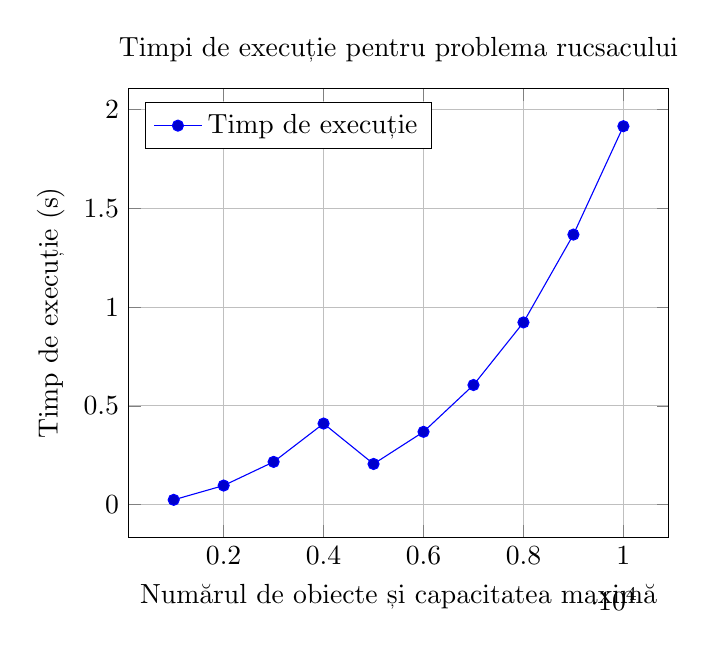
\begin{tikzpicture}
\begin{axis}[
    xlabel={Numărul de obiecte și capacitatea maximă},
    ylabel={Timp de execuție (s)},
    title={Timpi de execuție pentru problema rucsacului},
    legend pos=north west,
    grid=major
]
\addplot coordinates {
    (1000, 0.023719)
    (2000, 0.096105)
    (3000, 0.215982)
    (4000, 0.410176)
    (5000, 0.205441)
    (6000, 0.368231)
    (7000, 0.605409)
    (8000, 0.922518)
    (9000, 1.367393)
    (10000, 1.916276)
};
\addlegendentry{Timp de execuție}
\end{axis}
\end{tikzpicture}
\caption{Graficul timpilor de execuție pentru problema rucsacului}
\end{figure}

\subsection{Interpretare}

Analizând graficul timpilor de execuție pentru problema rucsacului, putem trage următoarele concluzii:

\begin{itemize}
    \item Timpii de execuție cresc în general odată cu creșterea numărului de obiecte și a capacității maxime a rucsacului. Aceasta este o așteptare normală, deoarece algoritmul de programare dinamică folosit are o complexitate de \(O(n * C)\), unde \(n\) este numărul de obiecte și \(C\) este capacitatea maximă a rucsacului.
    \item Observăm că până la testul 5, timpii de execuție cresc relativ liniar, dar începând cu testul 6, există o schimbare în tendința de creștere a timpului de execuție. Acest lucru poate fi explicat prin schimbarea intervalului valorilor și dimensiunilor obiectelor de la 1-1000 la 1-10000, care ar putea introduce o variabilitate suplimentară în calcul.
    \item În testele de la 6 la 10, timpii de execuție cresc semnificativ, sugerând că intervalul mai mare al valorilor și dimensiunilor obiectelor influențează performanța algoritmului.
    \item Testul 5 prezintă un timp de execuție mai mic decât testul 4, ceea ce poate indica o variabilitate în datele de intrare care permite o soluție mai rapidă în acel caz specific. Aceasta arată că în practică, chiar și pentru probleme similare, performanța poate varia în funcție de particularitățile setului de date.
\end{itemize}



\section{Rezultate și Concluzii}
Graficul timpilor de execuție pentru algoritmul rucsacului evidențiază câteva aspecte importante legate de performanța și eficiența acestuia în funcție de numărul de obiecte și capacitatea maximă a rucsacului:

\begin{itemize}
\item \textbf{Creșterea timpului de execuție în funcție de dimensiunea problemei:} Timpii de execuție cresc în general odată cu creșterea numărului de obiecte și a capacității maxime a rucsacului. Aceasta reflectă complexitatea algoritmului, care este O(n×C), unde n este numărul de obiecte și C este capacitatea rucsacului.
\item \textbf{Impactul intervalului valorilor și dimensiunilor obiectelor:} Observăm o schimbare semnificativă în timpii de execuție după testul 5, când intervalul valorilor și dimensiunilor obiectelor s-a schimbat de la 1-1000 la 1-10000. Aceasta sugerează că un interval mai mare de valori și dimensiuni poate introduce o variabilitate suplimentară care afectează performanța.
\item \textbf{Variabilitatea datelor de intrare:} Timpul de execuție mai mic pentru testul 5 comparativ cu testul 4 indică faptul că particularitățile setului de date pot influența semnificativ performanța. Deși în medie timpii cresc, există situații în care algoritmul poate funcționa mai eficient pentru anumite date.
\item \textbf{Scalabilitatea algoritmului:} Pe măsură ce dimensiunea problemei crește, timpii de execuție devin semnificativ mai mari. Aceasta subliniază importanța optimizării și a posibilei utilizări a tehnicilor de reducere a dimensiunii problemei sau de paralelizare pentru a gestiona probleme de foarte mari dimensiuni.
\end{itemize}

În concluzie, deși algoritmul de programare dinamică pentru problema rucsacului este eficient și asigură o soluție optimă, performanța sa este sensibilă la dimensiunea problemei și la caracteristicile specific ale datelor de intrare. Pentru aplicații practice, este esențială o evaluare atentă a acestor factori și, acolo unde este posibil, implementarea unor optimizări suplimentare.

\end{document}

